% MORPH — Core-MLP Lifecycle: Block-ELL · CMS pruning · ReMoE routing.
% Companion to morph_block.tex (the static forward view). Tells the TRAINING-LIFECYCLE story
% via the SwiGLU-MLP weight as a tile-grid evolving across phases.
%
% Verified against code (2026-06-07, subagent file:line audit):
%   - CMSBlockLinear dual-mode: dense [out,in] (cuBLAS F.linear) -> compact() -> Block-ELL values[R,K,16,16]+col_indices.
%   - tile_size B=16 (WMMA); R=out/16, C=in/16, K active block-cols/row, density=K/C.
%   - Block-ELL forward+backward Triton kernels are real (block_ell_forward/backward.py).
%   - block_ell_scope=all applies Block-ELL to prelude + core + coda SwiGLU MLPs (gate_up + down).
%   - ReMoE TileRouter: PEER product-key -> ReLU gate (activation_ratio), load-balance aux loss;
%     activation-conditioned (per-token), NOT keyed on the loop-iteration index.
% Compile: pdflatex morph_cms_lifecycle.tex

\documentclass[border=14pt]{standalone}
\usepackage[T1]{fontenc}
\usepackage{amsmath,amssymb}
\usepackage{tikz}
\usetikzlibrary{arrows.meta, fit, positioning, calc, backgrounds, decorations.pathreplacing}

% ── Palette (colorblind-safe) ────────────────────────────────────────────────
\definecolor{cbBlue}{HTML}{0072B2}
\definecolor{cbOrange}{HTML}{D55E00}
\definecolor{cbPurple}{HTML}{AA3377}
\definecolor{cbTeal}{HTML}{009E73}
\definecolor{fGray}{HTML}{EBEBEB}
\definecolor{bdr}{HTML}{555555}
\definecolor{stepC}{HTML}{2255AA}

\tikzset{
  ttl/.style={font=\normalsize\sffamily\bfseries},
  dsc/.style={font=\small\sffamily, align=center},
  nte/.style={font=\scriptsize\sffamily, align=center},
  tny/.style={font=\scriptsize\sffamily},
  A/.style={-{Stealth[length=3.4mm,width=2.8mm]}, line width=1.3pt, bdr},
  badge/.style={draw=#1, line width=0.8pt, rounded corners=2pt, fill=#1!15,
    text=#1!55!black, font=\scriptsize\sffamily\bfseries, inner sep=2.5pt},
}

% tile geometry
\def\ts{0.26}   % tile side
\def\tg{0.30}   % tile pitch (side + gap)
\def\gx{0.42}   % grid x-offset (centres the grid within the wider box)

% \celldraw{col}{row}{fill}{border} — one tile; rows go DOWN
\newcommand{\celldraw}[4]{%
  \draw[draw=#4, line width=0.4pt, fill=#3]
    ({\gx+#1*\tg},{-#2*\tg}) rectangle ++({\ts},{-\ts});}

\begin{document}
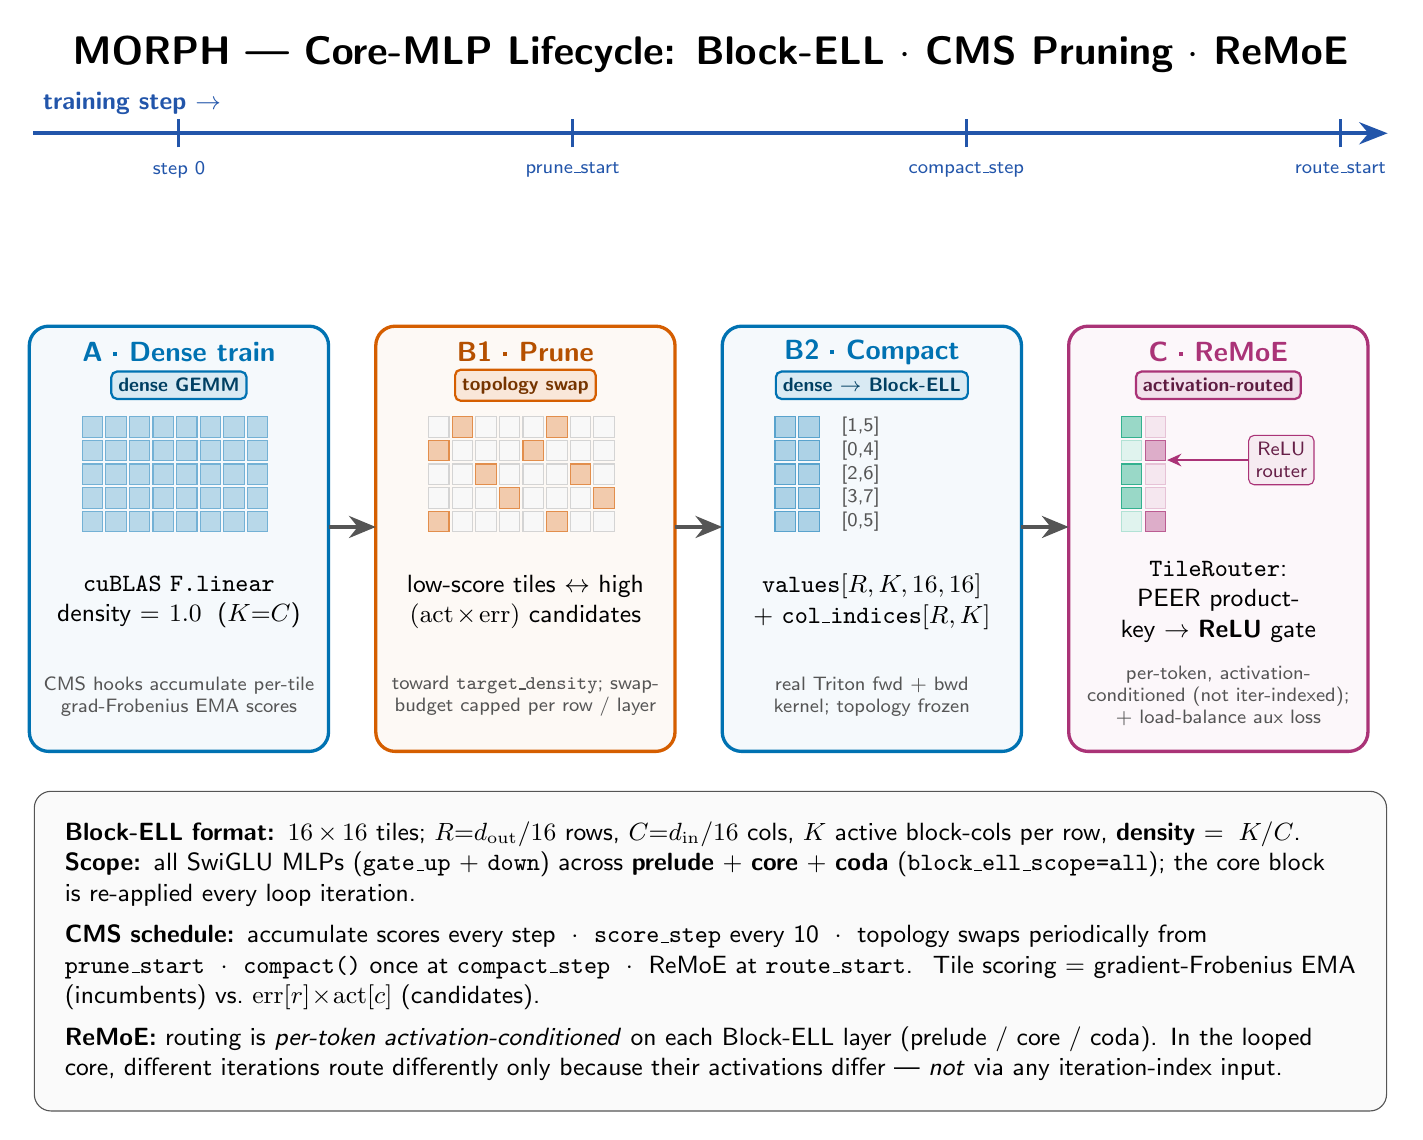
\begin{tikzpicture}

% box geometry: each phase box spans x in [-0.25, 3.55] (width 3.8), centre 1.65
\def\bxl{-0.25}\def\bxr{3.55}\def\bcx{1.65}
\def\bxt{1.15}\def\bxb{-4.25}

% =====================================================================
% TRAINING-STEP AXIS (top) — spans all four phase columns
% =====================================================================
\draw[-{Stealth[length=3.6mm,width=2.8mm]}, line width=1.4pt, stepC]
  (-0.2,3.6) -- (17.0,3.6);
\node[stepC, font=\small\sffamily\bfseries, anchor=south west] at (-0.2,3.72) {training step $\rightarrow$};
\foreach \x/\lab in {1.65/{step 0}, 6.65/{prune\_start}, 11.65/{compact\_step}, 16.4/{route\_start}}{
  \draw[stepC, line width=1.1pt] (\x,3.42) -- (\x,3.78);
  \node[stepC, tny, anchor=north] at (\x,3.36) {\lab};
}

% =====================================================================
% PHASE A — DENSE TRAIN  (origin x=0)
% =====================================================================
\begin{scope}[xshift=0cm]
  \draw[draw=cbBlue, very thick, rounded corners=7pt, fill=cbBlue!4]
    (\bxl,\bxt) rectangle (\bxr,\bxb);
  \node[ttl, text=cbBlue] at (\bcx,0.82) {A · Dense train};
  \node[badge=cbBlue] at (\bcx,0.40) {dense GEMM};
  \foreach \r in {0,...,4}\foreach \c in {0,...,7}{ \celldraw{\c}{\r}{cbBlue!28}{cbBlue!55} }
  \node[dsc, text width=3.5cm] at (\bcx,-2.35)
    {\texttt{cuBLAS F.linear}\\ density $=1.0$ \;($K{=}C$)};
  \node[nte, text=bdr, text width=3.5cm] at (\bcx,-3.55)
    {CMS hooks accumulate per-tile grad-Frobenius EMA scores};
\end{scope}

% =====================================================================
% PHASE B1 — PRUNE  (origin x=4.4)
% =====================================================================
\begin{scope}[xshift=4.4cm]
  \draw[draw=cbOrange, very thick, rounded corners=7pt, fill=cbOrange!4]
    (\bxl,\bxt) rectangle (\bxr,\bxb);
  \node[ttl, text=cbOrange!85!black] at (\bcx,0.82) {B1 · Prune};
  \node[badge=cbOrange] at (\bcx,0.40) {topology swap};
  \foreach \r in {0,...,4}\foreach \c in {0,...,7}{ \celldraw{\c}{\r}{fGray!35}{bdr!25} }
  \foreach \r/\c in {0/1,0/5, 1/0,1/4, 2/2,2/6, 3/3,3/7, 4/0,4/5}{
    \celldraw{\c}{\r}{cbOrange!32}{cbOrange!70} }
  \node[dsc, text width=3.5cm] at (\bcx,-2.35)
    {low-score tiles $\leftrightarrow$ high $(\mathrm{act}\!\times\!\mathrm{err})$ candidates};
  \node[nte, text=bdr, text width=3.5cm] at (\bcx,-3.55)
    {toward \texttt{target\_density}; swap-budget capped per row / layer};
\end{scope}

% =====================================================================
% PHASE B2 — COMPACT  (origin x=8.8)
% =====================================================================
\begin{scope}[xshift=8.8cm]
  \draw[draw=cbBlue, very thick, rounded corners=7pt, fill=cbBlue!4]
    (\bxl,\bxt) rectangle (\bxr,\bxb);
  \node[ttl, text=cbBlue] at (\bcx,0.82) {B2 · Compact};
  \node[badge=cbBlue] at (\bcx,0.40) {dense $\to$ Block-ELL};
  \foreach \r in {0,...,4}\foreach \c in {0,1}{ \celldraw{\c}{\r}{cbBlue!32}{cbBlue!65} }
  \foreach \r/\a/\b in {0/1/5, 1/0/4, 2/2/6, 3/3/7, 4/0/5}{
    \node[tny, text=bdr, anchor=west] at ({\gx+2*\tg+0.12},{-\r*\tg-0.5*\ts}) {[\a,\b]};}
  \node[dsc, text width=3.5cm] at (\bcx,-2.35)
    {\texttt{values}$[R,K,16,16]$\\ $+$ \texttt{col\_indices}$[R,K]$};
  \node[nte, text=bdr, text width=3.5cm] at (\bcx,-3.55)
    {real Triton fwd $+$ bwd kernel; topology frozen};
\end{scope}

% =====================================================================
% PHASE C — ReMoE ROUTING  (origin x=13.2)
% =====================================================================
\begin{scope}[xshift=13.2cm]
  \draw[draw=cbPurple, very thick, rounded corners=7pt, fill=cbPurple!4]
    (\bxl,\bxt) rectangle (\bxr,\bxb);
  \node[ttl, text=cbPurple] at (\bcx,0.82) {C · ReMoE};
  \node[badge=cbPurple] at (\bcx,0.40) {activation-routed};
  \foreach \r/\on in {0/1, 1/0, 2/1, 3/1, 4/0}{
    \ifnum\on=1
      \celldraw{0}{\r}{cbTeal!40}{cbTeal!80}\celldraw{1}{\r}{cbPurple!12}{cbPurple!30}
    \else
      \celldraw{0}{\r}{cbTeal!12}{cbTeal!30}\celldraw{1}{\r}{cbPurple!40}{cbPurple!80}
    \fi}
  \node[draw=cbPurple, rounded corners=2pt, fill=cbPurple!10, font=\scriptsize\sffamily,
        align=center, text=cbPurple!60!black, inner sep=2.5pt] (rt) at (2.45,-0.55) {ReLU\\router};
  \draw[-{Stealth[length=1.8mm,width=1.6mm]}, cbPurple, line width=0.8pt]
    (rt.west) -- ({\gx+2*\tg-0.02},-0.55);
  \node[dsc, text width=3.5cm] at (\bcx,-2.35)
    {\texttt{TileRouter}: PEER product-key $\to$ \textbf{ReLU} gate};
  \node[nte, text=bdr, text width=3.5cm] at (\bcx,-3.55)
    {per-token, activation-conditioned (not iter-indexed); $+$ load-balance aux loss};
\end{scope}

% ── progression arrows between phase boxes ───────────────────────────
\draw[A] (3.55,-1.4) -- (4.15,-1.4);
\draw[A] (7.95,-1.4) -- (8.55,-1.4);
\draw[A] (12.35,-1.4) -- (12.95,-1.4);

% =====================================================================
% FACTS PANEL (bottom, full width)
% =====================================================================
\node[draw=bdr, rounded corners=6pt, fill=fGray!25, inner sep=11pt,
      align=left, font=\small\sffamily, text width=16.4cm, anchor=north]
      (facts) at (8.4,-4.75) {%
  \textbf{Block-ELL format:} $16\!\times\!16$ tiles; $R{=}d_{\mathrm{out}}/16$ rows, $C{=}d_{\mathrm{in}}/16$ cols,
  $K$ active block-cols per row, \textbf{density $=K/C$}.\quad
  \textbf{Scope:} all SwiGLU MLPs (\texttt{gate\_up} $+$ \texttt{down}) across \textbf{prelude $+$ core $+$ coda}
  (\texttt{block\_ell\_scope=all}); the core block is re-applied every loop iteration.\\[4pt]
  \textbf{CMS schedule:} accumulate scores every step \;$\cdot$\; \texttt{score\_step} every 10 \;$\cdot$\; topology swaps periodically from \texttt{prune\_start}
  \;$\cdot$\; \texttt{compact()} once at \texttt{compact\_step} \;$\cdot$\; ReMoE at \texttt{route\_start}.
  \;Tile scoring $=$ gradient-Frobenius EMA (incumbents) vs.\ $\mathrm{err}[r]\!\times\!\mathrm{act}[c]$ (candidates).\\[4pt]
  \textbf{ReMoE:} routing is \emph{per-token activation-conditioned} on each Block-ELL layer (prelude / core / coda).
  In the looped core, different iterations route differently only because their activations differ --- \emph{not} via any iteration-index input.};

% ── Title ────────────────────────────────────────────────────────────
\node[font=\Large\sffamily\bfseries, anchor=south] at (8.4,4.25)
  {MORPH --- Core-MLP Lifecycle: Block-ELL $\cdot$ CMS Pruning $\cdot$ ReMoE};

\end{tikzpicture}
\end{document}
